
\section{Flapping Wing simulation}

An application example of \acrshort{precice}-\acrshort{mbdyn} coupling in the study of \acrshort{fsi} problems can be found in \cite{heathcote2008effect}, in which the effect of spanwise wing flexibility on thrust, lift and propulsive efficiency of a rectangular wing oscillating in pure heave is analyzed by means of water tunnel experiments.

The study shows that, for some oscillating frequencies, a degree of spanwise flexibility yields a small
increase in thrust coefficient and a small decrease in power-input requirement, resulting in higher overall efficiency.

\subsection{Experimental setup}

Before describing the \acrshort{fsi} model and the simulation, it is necessary to briefly introduce the experimental setup.

The study considers three types of rectangular wings, with profile \textit{naca 0012} and with different section properties, as shown in Figure~\ref{fig:profiles0012}. The section labeled (i) is considered \textit{inflexible}, the one labeled (ii) is considered \textit{flexible} and the last one \textit{highly flexible}.

\begin{figure}[htbp!]
	\centering
	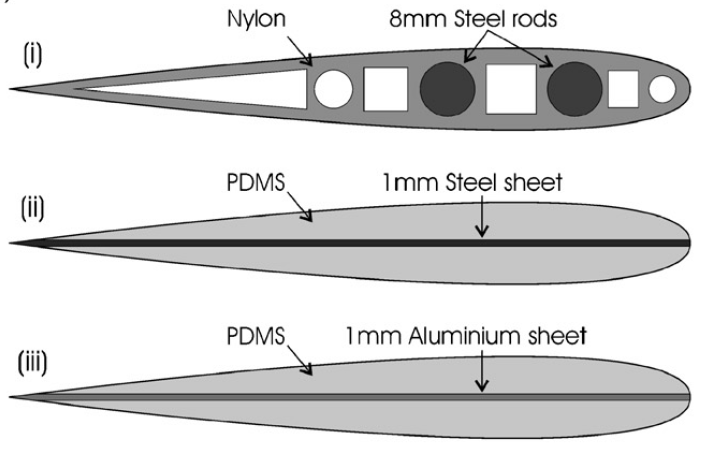
\includegraphics[width=0.7\textwidth]{images/profiles0012}
	\caption{wing section properties (image taken from \cite{heathcote2008effect})}
	\label{fig:profiles0012}
\end{figure}

Each wing has the following dimensions: $100$\si{mm} chord and $300$\si{mm} span.

The experimental setup is shown in Figure~\ref{fig:0012exp}. The displacement of the root section is given by $s = a_{ROOT} \cos(\omega t)$, where $a_{ROOT} = 0.175c$. The flow velocity $U_0$ is in the range $1-3$\si{m.s^{-1}}. The following dimensionless parameters are considered:

\begin{itemize}
	\item $Re = \frac{\rho U_0 c}{\mu}$: Reynolds number
	\item $k_G = \frac{\pi f c}{U_0}$: Garrick reduced frequency
	\item $S_r = \frac{2f a_{MID}}{U_0}$: Strouhal number at mid-span
\end{itemize}

\begin{figure}[htbp!]
	\centering
	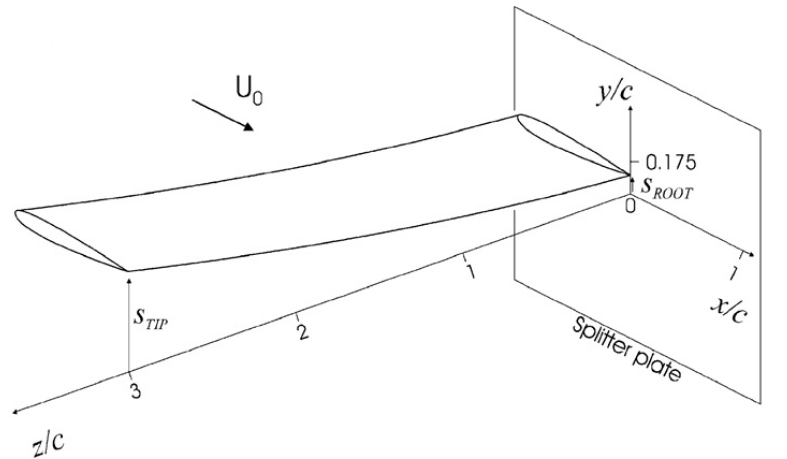
\includegraphics[width=0.7\textwidth]{images/naca0012_exp}
	\caption{experimental setup (image taken from \cite{heathcote2008effect})}
	\label{fig:0012exp}
\end{figure}

Experiments are carried out for the three types of wings in the following ranges: $Re=1\cdot10^4-3\cdot10^4$ and $k_G=0-7$.

The results give information concerning the average thrust coefficient $C_T = \frac{T}{\frac{1}{2}\rho U_0^2c}$ over a finite number of cycles and the mean power input coefficient $\bar{C}_P = \frac{\bar{F_y v}}{\frac{1}{2}\rho U_0^3c}$.

Besides, information concerning the ratio $\frac{a_{TIP}}{a_{ROOT}}$ and tip phase lag $\phi$ are given.

\subsection{Simulation setup}

The experimental setup described in \cite{heathcote2008effect} has been replicated in a \acrshort{fsi} simulation using \acrshort{mbdyn} as structural solver and OpenFOAM as \acrshort{cfd} solver.

\subsubsection{Fluid domain}

The fluid domain is represented by a box of size $1.5\times 0.6\times 0.5$\si{m}, as represented in Figure~\ref{fig:hc-mesh}. The boundary conditions are:

\begin{itemize}
    \item constant inlet velocity for the face at $x=-0.25$\si{m},
    \item constant pressure for the face at $x=1.25$\si{m},
    \item symmetry plane at the root of the wing ($z=0$),
    \item slip walls for the other external surfaces,
    \item no-slip wall for the wing surface.
\end{itemize}

The naca0012 wing has been drawn in \textit{Salome} and exported in OpenFOAM as \textit{.stl} file. The mesh has been built with the tool \textit{snappyHexMesh} and it is composed of 218451 cells. 



\begin{figure}[htbp!]
	\centering
	\begin{subfigure}{.75\textwidth}
		\centering
		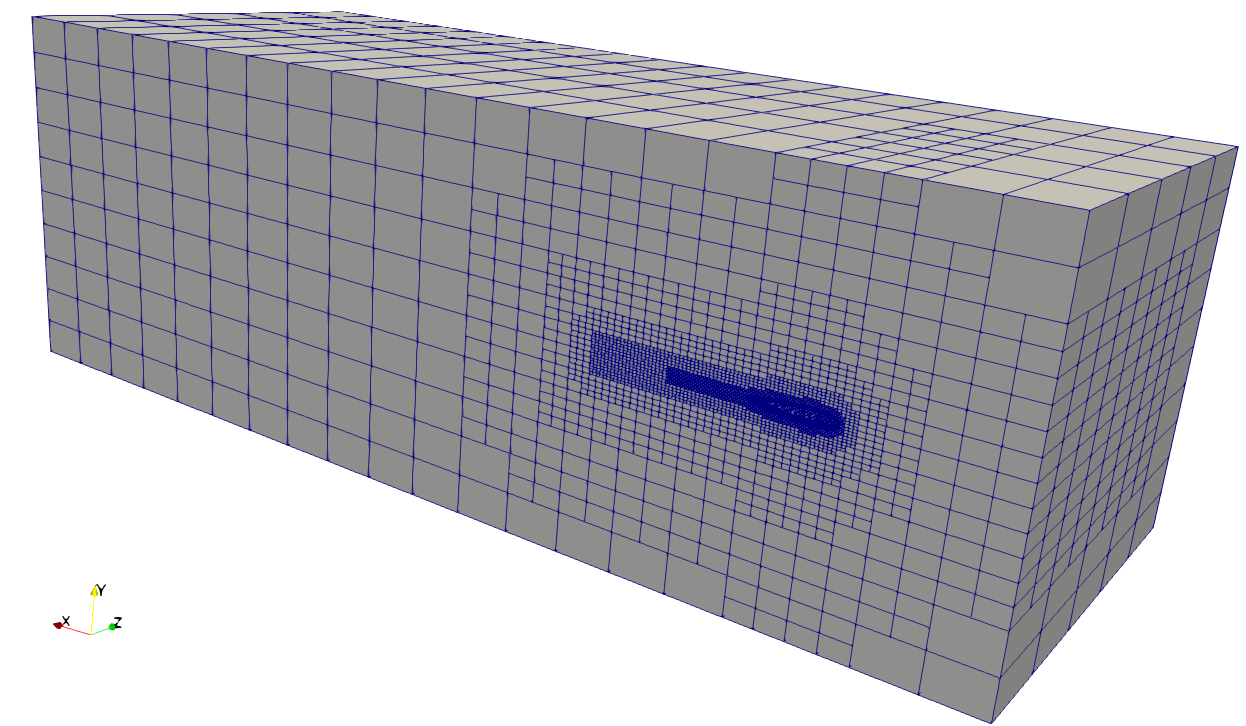
\includegraphics[width=.99\linewidth]{images/heathcote/dom03.png}
		\caption{mesh bounding box}
		%\label{fig:undist}
	\end{subfigure}
	\newline
	
	\centering
	\begin{subfigure}{.75\textwidth}
		\centering
		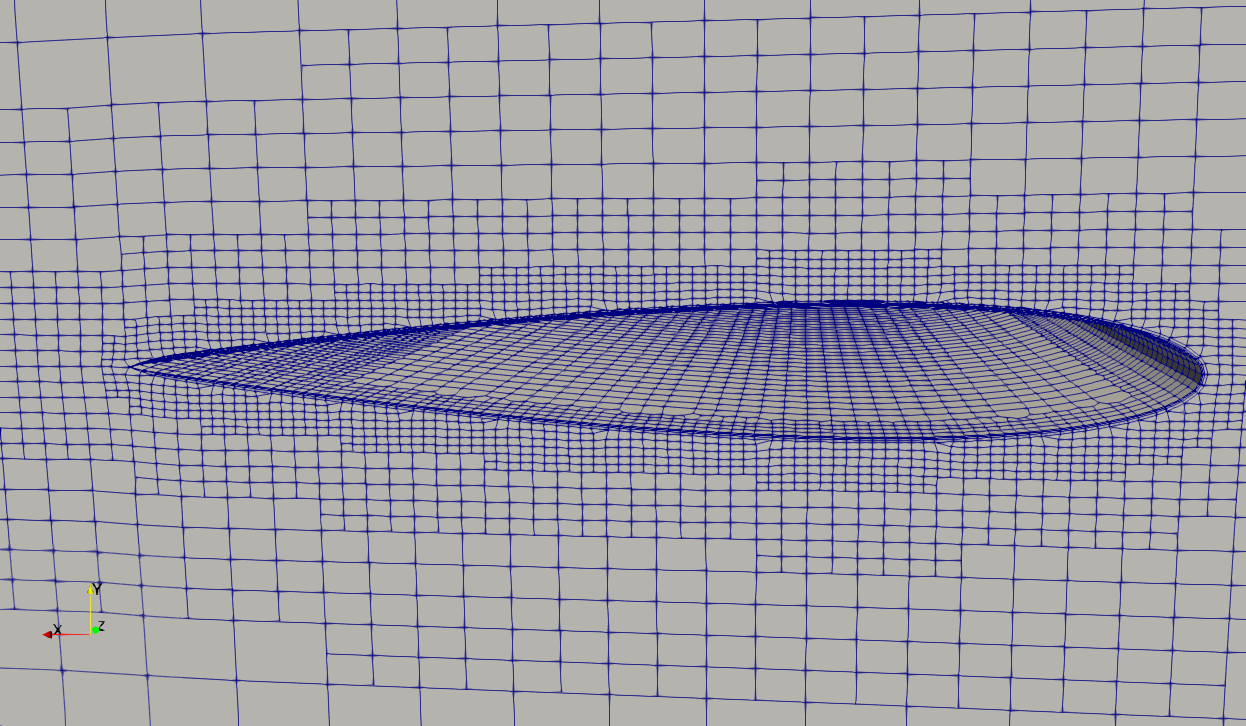
\includegraphics[width=.99\linewidth]{images/heathcote/dom02.png}
		\caption{wing detail}
		%\label{fig:dist}
	\end{subfigure}
	\caption{fluid mesh}
	\label{fig:hc-mesh}
\end{figure}



\subsubsection{Interface}

The same naca0012 profile drawn in Salome has been used to generate the interface mesh for the \texttt{external structural mapping} of MBdyn. The interface mesh is composed of 1286 cells (1200 quadrangles and 86 triangles), as shown in Figure~\ref{fig:hc-interface}.

\begin{figure}[htbp!]
	\centering
	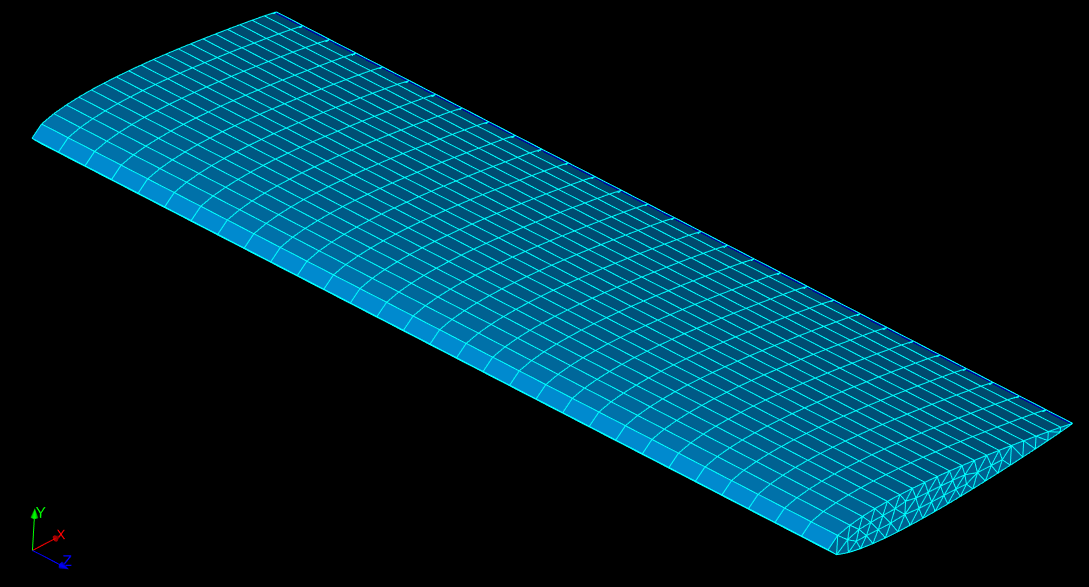
\includegraphics[width=0.75\textwidth]{images/heathcote/interface01.png}
	\caption{interface mesh}
	\label{fig:hc-interface}
\end{figure}


\subsubsection{Structural domain}

The structural model is composed of 10 MBDyn \texttt{beam} elements. Considering the \textit{flexible} (or the \textit{highly flexible}) structure, the stiffness of the wing can be considered completely given by the 1\si{mm} metal plate, as the PDMS, with a Young modulus of $360\div870$ \si{kPa} would contribute with only a small fraction of the overall stiffness.

The stiffness matrix of each beam element is given in Equation~\ref{eq:hc-stiff}, in which $w$ represents the chord and $h$ the metal thickness.

\begin{equation}
    \begin{bmatrix} Ewh &  & 0 & \ldots &  & 0 \\
                          & Gwh &  & & & &  \\
                          & & Gwh & & & \\
                          & & & G\frac{1}{3}wh^3 & & \vdots \\
                          & &  sym. & & E\frac{1}{12}wh^3 &  \\
                          & & & & & E\frac{1}{12}hw^3
    \end{bmatrix} 
    \label{eq:hc-stiff}
\end{equation}

At each of the 21 nodes of the structure there is a \texttt{body} element attached, carrying the mass of the corresponding chunk of beam (both metal and PDMS).

The wing motion is achieved by means of a \texttt{total pin joint} element attached to the root of the wing, which moves the root \texttt{node} with a $\sin(\omega t)$ law along the $y$ direction. The motion starts with a ramp of the  kind $\frac{1}{2}\left(1-\cos\left(\frac{t}{\tau}\right)\right)$ in order to ease convergence.

\subsubsection{Coupling}

The main data concerning the coupling between the fluid solver and the structural solver  are given in Table~\ref{table:hc-coupling}:


\begin{table}[!htb]
	\begin{center}
		\begin{tabular}{ l c  l| c } 
			\multicolumn{3}{c|}{parameter} & value   \\ 
			\hline
			simulation time  & $t$& \si{s} & 2      \\
			step size & $\Delta t$ & \si{s} & $10^{-3}$   \\
			\hline
			coupling scheme & & & serial implicit  $S\rightarrow F$  \\
			coupling algorithm & & &  IQN-ILS  \\
			displacement rel. convergence limit & & & $10^{-3}$ \\
			force rel. convergence limit &&  & $10^{-3}$  \\
      		interface mesh mapping & & & Nearest neigh. and RBF  \\
			
		\end{tabular}
	\end{center}
	\caption{naca0012: coupling parameters}
	\label{table:hc-coupling}
\end{table}

Different experiments have been carried out considering different parameters. For example, a shorter time step is beneficial for a better mesh displacement, at the expense of a longer simulation time. At the same time, convergence limits have an obvious impact on the simulation time, as more iterations are required in order to reach a lower convergence limit.

Finally, also mesh mapping strategy (see Section \ref{sec:data-mapping}) influence the simulation quality and time: \textit{nearest-neighbor} is faster but can be detrimental for mash movement, on the other side, the \acrfull{rbf} mapping gives better results, but for larger grids ($\approx4000$ points) the computational cost of the mapping becomes relevant. Moreover, it needs to be tuned.

\subsection{Results}

Due to resource constraints, only some preliminary results have been carried out.  